\documentclass[12pt, twoside]{report}
%--------------- Paquetes -----------------------
%------- [Para formato general] --------------


\usepackage{float}          % Para manejo de objetos en entornos float   
\usepackage{geometry}       % Para añadir márgenes 

\usepackage{fancyhdr}       % Para encabezados
\usepackage{pdflscape}      % Permite la rotación de páginas
\usepackage{rotating}       % Permite el cambio de orientación
\usepackage{helvet}         % Para letra helvética similar a arial
\renewcommand{\familydefault}{\sfdefault}
\usepackage[spanish]{babel} % Para comandos en español
\usepackage{titlesec}       % Para sección de títulos

%------- [Para tablas y figuras] ----------------
\usepackage{graphicx}       % Para manejo de graficos
\usepackage{booktabs}       % Para mejorar la calidad de las tablas
\usepackage{longtable}      % Para tablas extensas
\usepackage{tabularx}       % Adicional al paquete tabular
\usepackage{multirow}       % Para combinar filas
\usepackage{makecell}       % Para formato de celdas
\usepackage{epstopdf}       % Convierte imagenes EPS a PDF
\epstopdfsetup{update}      
\usepackage{pdfpages}       % Para añadir documentos pdf

%------- [Para referencias] -------------------
\usepackage[backend=biber, style=apa]{biblatex}   % Referencias APA
\addbibresource{Referencias.bib}
\usepackage{csquotes}       % Para citaciones avanzadas
\usepackage{appendix}       % Añade sección de apéndice
\usepackage{tocloft}        % Para tabla de contenidos

%------- [Para fórmulas] -------------------
\usepackage{amsmath,amssymb,amsfonts} % Para fórmulas matemáticas
\usepackage{nomencl}        % Produce lista de nomenclaturas
\usepackage[version=4,arrows=pgf-filled, textfontname=mathsf]{mhchem}                    % Para fórmulas químicas 

%------- [FORMATEO DE PÁGINA] ------------

\geometry{
    a4paper, 
    left=3.5cm,
    right=2.5cm,
    bottom=2.5cm,
    top=2.5cm,
    headheight=2.5cm
    }

%------- [FORMATEO DE SUBTÍTULOS Y NUMERACIÓN] ------------
\usepackage{caption}
\usepackage{subcaption}
\captionsetup{font=small}
\captionsetup{
    labelsep=newline,
    labelfont=normalfont,
    textfont=it,
    justification=raggedright,
    singlelinecheck=false
}
\DeclareCaptionLabelSeparator{newline}{\\} %para quitar el punto y coma al final de la etiqueta, Por ejemplo: figura 1  
\captionsetup{labelsep=newline} %Ubica el contenido de la etiqueta en la segunda linea, en lugar de la primera. 

%------ Conservación de la numeración ---------
\usepackage{chngcntr}               % Mantiene la numeración 
\counterwithout{figure}{chapter}    % Mantiene la numeración en figuras
\counterwithout{table}{chapter}     % Mantiene la numeración en tablas

 %------- [FORMATEO DE CAPÍTULOS] ------------
\titleformat{\chapter}[hang]{\Large\bfseries}{\Roman{chapter}.}{1em}{}
\titlespacing*{\chapter}
{0cm}                   % Margen izquierdo 
{0cm}                   % Espacio antes del título  
{0.5cm}                 % Espacio después del título 

% Para mantener secciones, figuras, tablas y ecuaciones en números arábigos
\renewcommand{\thesection}{\arabic{chapter}.\arabic{section}}
\renewcommand{\thesubsection}{\arabic{chapter}.\arabic{section}.\arabic{subsection}}
\renewcommand{\theequation}{\arabic{chapter}.\arabic{equation}}
\renewcommand{\thefigure}{\arabic{figure}}
\renewcommand{\thetable}{\arabic{table}}

 %------- [FORMATEO DE ANEXOS (APÉNDICES)] ------------

\newcounter{annex}
\renewcommand{\theannex}{\Alph{annex}}

% Comando para definir la sección de anexos
\newcommand{\sectionannex}[1]{%
    \refstepcounter{annex}
    \setcounter{figure}{0}
    \setcounter{table}{0}
    \clearpage
    \thispagestyle{empty}
    \vspace*{\stretch{1}}
    \begin{center}
        \begin{minipage}{\textwidth}
            \centering
            {\LARGE\bfseries Anexo \theannex\par}
            \vspace{1.5ex}
            {\large\itshape #1\par}
        \end{minipage}
    \end{center}
    \vspace*{\stretch{1}}
    \clearpage
}

% ------------------- [FORMATEO DE CUERPO DEL DOCUMENTO Y ADICIONALES ] -------------------

\setcounter{secnumdepth}{3}
\setlength{\parskip}{1\baselineskip}
\setlength{\parindent}{1cm}
\makenomenclature
\renewcommand{\nomname}{List of Abbreviations}
\renewcommand{\bibname}{References}
\addto\captionsspanish{\renewcommand{\tablename}{Tabla}}
\addto\captionsspanish{\renewcommand{\listtablename}{Índice de tablas}}

% Encabezados
\fancyhf{}
\pagestyle{fancy}
\fancyfoot[C]{\thepage}
\fancyhead{}
\renewcommand{\headrulewidth}{0pt}

 %-----------------------------------------------------------------
% Quitar el comentario de \includeonly para cargar una seccion en específico

%\includeonly{capítulos/Introducción}

\begin{document}
% Incluye tu portada en formato pdf
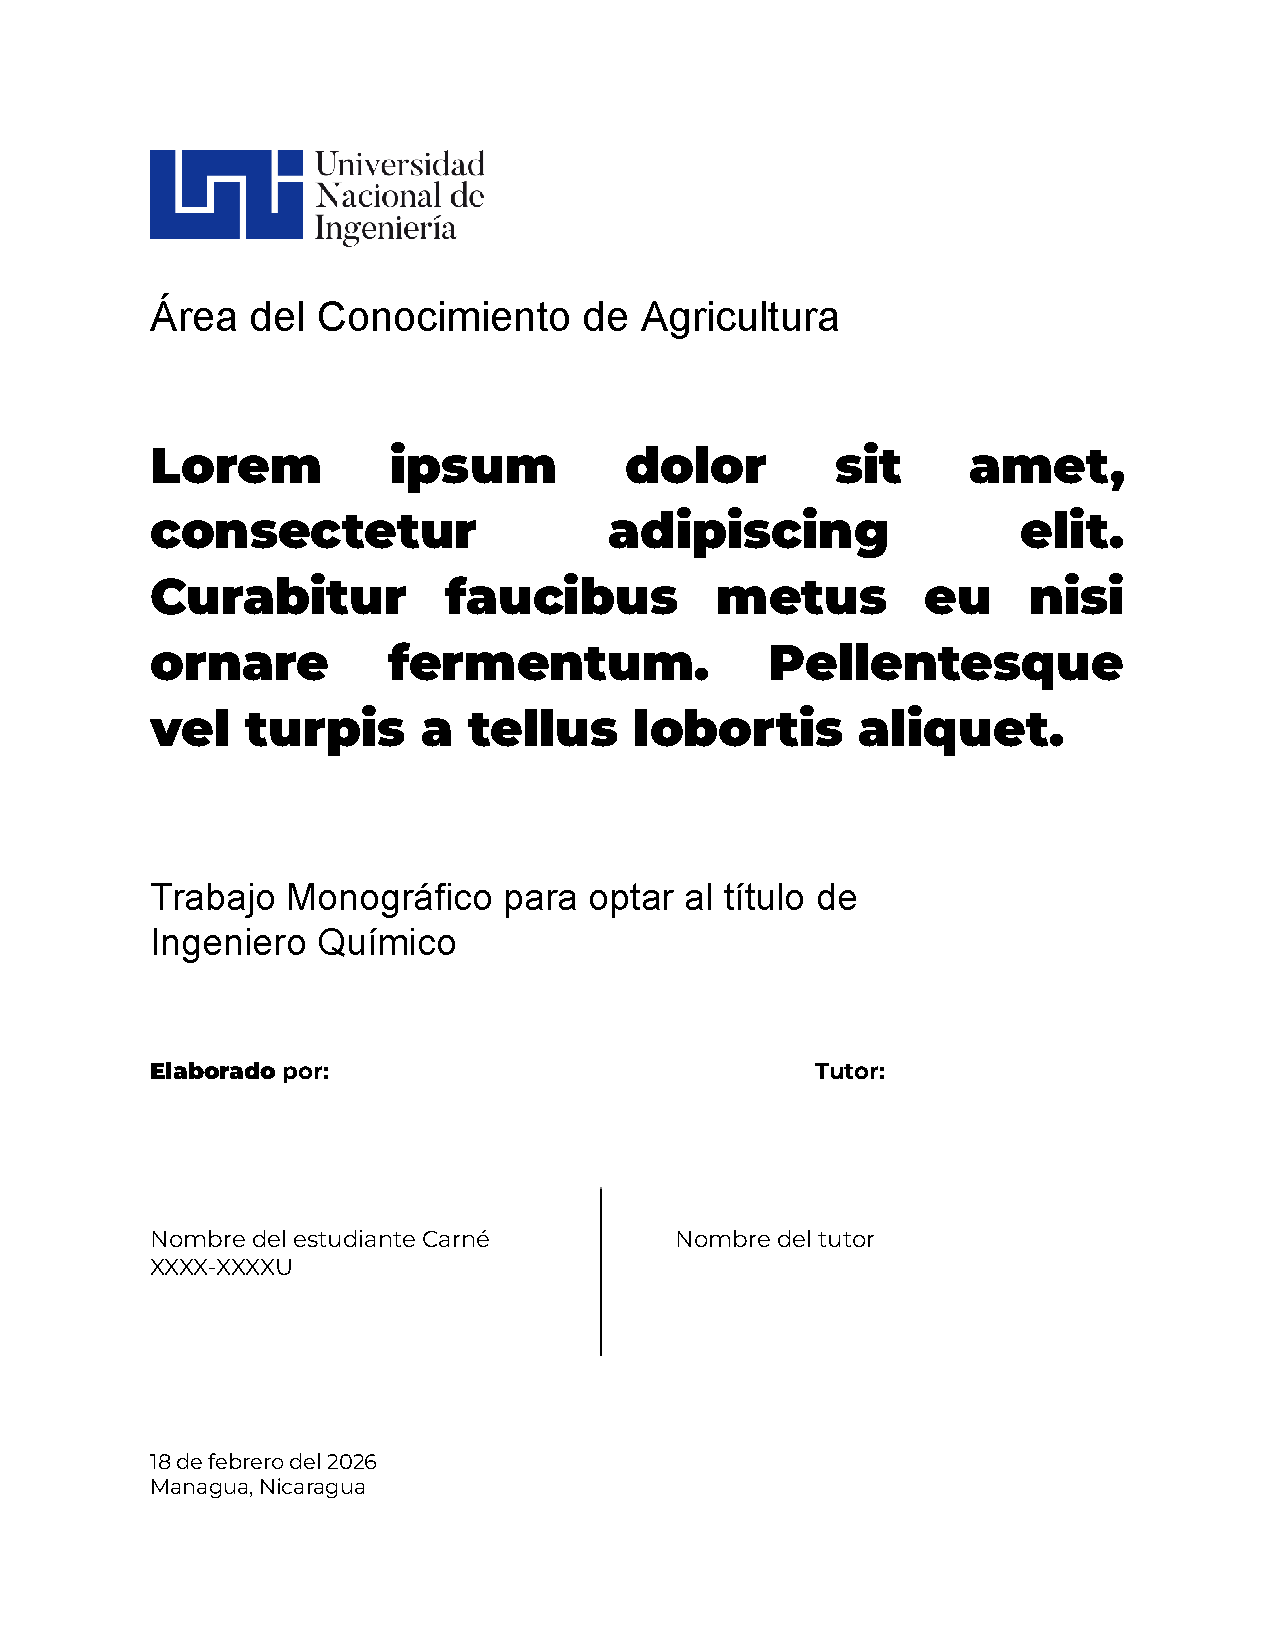
\includepdf[pages=-]{Preambulo/PORTADA DE MONOGRAFIA.pdf}


\pagenumbering{roman} % Para el conteo de las primeras secciones del doc en números romanos. 
\include{Preambulo/Agradecimientos}
\chapter*{Dedicatoria}

Lorem ipsum dolor sit amet, consectetur adipiscing elit. Curabitur faucibus metus eu nisi ornare fermentum. Pellentesque vel turpis a tellus lobortis aliquet. Phasellus turpis nulla, semper finibus enim ac, scelerisque congue nibh. Cras ultrices imperdiet sapien, sit amet porta nulla porta ac.
\chapter*{RESUMEN}
\addcontentsline{toc}{chapter}{RESUMEN} %Añade el capítulo a la tabla de contenidos

Lorem ipsum dolor sit amet, consectetur adipiscing elit. Curabitur faucibus metus eu nisi ornare fermentum. Pellentesque vel turpis a tellus lobortis aliquet. Phasellus turpis nulla, semper finibus enim ac, scelerisque congue nibh. Cras ultrices imperdiet sapien, sit amet porta nulla porta ac. Curabitur ipsum ligula, vehicula eu ornare sit amet, pharetra tincidunt turpis. Donec non mi ut eros tincidunt suscipit quis eu nisl. Vestibulum at hendrerit massa. Vivamus vitae enim ut velit consectetur tincidunt. Nulla imperdiet maximus magna id pellentesque. Duis non lorem ac nulla maximus tincidunt eu non dui. Pellentesque habitant morbi tristique senectus et netus et malesuada fames ac turpis egestas.
\include{Preambulo/Opinion_Tutor}

\newpage
\tableofcontents
\newpage
\listoffigures
\newpage
\listoftables
\clearpage

\pagenumbering{arabic} % Para el contenido del documento en números arábigos 
\chapter{INTRODUCCIÓN}
\label{cap:Introduccion} %Añadir etiquetas en caso de mencionar capítulos en el texto. 

Nunc ac velit sodales, molestie augue quis, dignissim odio. Nunc tempus neque id turpis placerat venenatis. Pellentesque imperdiet nisi a dolor euismod vehicula. Nulla vehicula luctus metus, id consectetur sem sagittis eu. Morbi cursus fringilla ultricies. Curabitur nibh leo, feugiat maximus sodales sed, lacinia at lectus. Nulla volutpat rutrum tortor in venenatis. Phasellus sed vehicula ante. Maecenas ullamcorper, nisi non elementum ornare, nulla justo scelerisque diam, vitae vehicula nunc lectus id lacus. Pellentesque habitant morbi tristique senectus et netus et malesuada fames ac turpis egestas. Phasellus et arcu nulla. Donec non consequat purus, ac finibus mauris. Fusce pharetra volutpat elit. Suspendisse potenti. Sed sed porttitor felis, vel venenatis enim.
\chapter{OBJETIVOS}

\section{Objetivo General}
Suspendisse ornare magna et ligula vestibulum, eget mollis justo mattis. Nullam ut tempor ante, sit amet feugiat nisi. Mauris accumsan dolor in congue commodo.

\section{Objetivos especificos}
\begin{itemize}
    \item Objetivo especifico 1
    \item Objetivo especifico 2
    \item Objetivo especifico 3
\end{itemize}

\chapter{MARCO TEORICO}

\section{Tecnologia de membranas}
\subsection{Aspectos generales de la separacion por membranas}

Existen muchas definiciones para una membrana, sin embargo, de forma general, se define como una barrera delgada, situada entre dos fases o medios, lo que permite el paso selectivo de uno o más constituyentes de un medio a otro, en presencia de una fuerza impulsora apropiada, mientras se retiene el resto \parencite[p.~3]{Pabby2015} 

% ------------ Comando para insercion de figuras ------------------
\begin{figure}[ht]
\caption{Esquema general de un sistema de membrana. Tomado de Drioli, et al. (2018) \textit{Membrane Engineering} (P.2) DE GRUYTER. Figura 1.2}
\centering
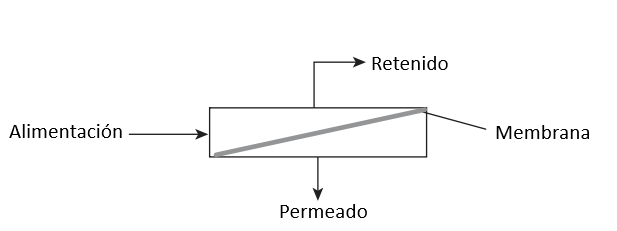
\includegraphics[width = 1\textwidth]{Figuras/esquema general de sistemas de membrana.png}
\label{fig:sep_membranas}
\end{figure}

De forma general, un sistema de membranas está conformado por cuatros componentes: una corriente de alimentación, una membrana, una corriente de permeado, que contiene las especies que han pasado a través de la membrana y una corriente de retenido o residuo (también denominado concentrado), que contiene especies que han sido excluidas o retenidas, y que no han pasado a través de la estructura de la membrana \parencite[p~8]{Singh2014}. La representación esquemática general de un sistema de membrana se muestra en la Figura \ref{fig:sep_membranas} con sus cuatro componentes.

La eficiencia de la separación en un sistema de membranas depende de algunas variables como el tipo de membrana, el modelo de difusión, fuerza impulsora, obstrucción en la membrana, etc., sin embargo, de forma general, la eficiencia de la separación puede ser cuantificada mediante el coeficiente de rechazo (R) que indica la habilidad de separación del proceso de membrana y se puede obtener mediante la Ecuación \ref{eq:RechazoMembrana} donde C1 representa la concentración del soluto en la alimentación del sistema y C2 representa la concentración del producto \parencite[p~13]{Singh2014} 

% ------------ Comando para insercion de ecuaciones ---------------
\begin{equation}
R = \frac{C_1 - C_2}{C_1} \times 100
\label{eq:RechazoMembrana}
\end{equation}

\subsection{Procesos de separación por membrana}
Los procesos de separación por membrana se pueden clasificar de manera general en función de su fuerza impulsora, ya sea debido a un gradiente de presión, temperatura, concentración, potencial eléctrico o vacío.

Los procesos impulsados por la presión se muestran en la Tabla \ref{tab:procesos de membrana}, donde las principales diferencias entre un proceso y otro son las presiones transmembrana con las que se operan para aumentar la velocidad del proceso de transporte y el rango de tamaño de partículas o solutos que son separados. Los procesos de Microfiltración (MF) se caracterizan por ser usualmente procesos de clarificación que separan las moléculas y partículas en base a su tamaño y solubilidad \parencite[p~7]{Nath2017}. Además, los procesos MF son los que tienen un menor requerimiento energético, en comparación con los demás procesos descritos en la Tabla \ref{tab:procesos de membrana}, debido a que las membranas utilizadas poseen mayores tamaños de poros, lo que permite que se puedan operar a menores presiones.

%-------------- Comando para tablas -------------------------

\begin{table}[ht]
\small    
\caption{Procesos de membrana impulsados por la presión}
    \centering
    \begin{tabular}{p{4cm} p{4cm} p{4cm} p{4cm}}
         \toprule
        Proceso de membrana & Presión transmembrana (bar) & Permeado & Retenido \\
         \midrule
        Microfiltración & 1 - 2 & Solutos disueltos, agua & Partículas retenidas, agua \\
        Ultrafiltración & 1 - 5 & Pequeñas moléculas, agua & Polímeros, proteínas, coloides particulados \\
        Nanofiltración & 5 - 15 & Iones monovalentes, agua & Pequeñas moléculas, sales divalentes \\
        Ósmosis inversa & 15 - 100 & Agua, pequeños solventes polares, sales & Todos los solutos, agua \\
         \bottomrule
    \end{tabular}
    \label{tab:procesos de membrana}
\end{table}
\small \textbf{Nota:} Traducido de Membrane Technology in Separation Science (P. 6) de M. Purkait, R. Singh (2008). CRC Press y Membrane separation Processes (P.7) de K. Nath (2017) PHI Learning Private Limited.

\include{capítulos/Metodología}
\chapter{RESULTADOS Y DISCUSION}

Nunc ac velit sodales, molestie augue quis, dignissim odio. Nunc tempus neque id turpis placerat venenatis. Pellentesque imperdiet nisi a dolor euismod vehicula. Nulla vehicula luctus metus, id consectetur sem sagittis eu. Morbi cursus fringilla ultricies. Curabitur nibh leo, feugiat maximus sodales sed, lacinia at lectus. 
\chapter{CONCLUSIONES}

Pellentesque habitant morbi tristique senectus et netus et malesuada fames ac turpis egestas. Vestibulum dignissim felis quis elit iaculis condimentum a condimentum sem. Nunc vehicula eu ante eu commodo. Vestibulum mauris turpis, rutrum et ornare et, laoreet sed metus. Vestibulum scelerisque, mi eu dapibus pretium, ipsum justo vehicula velit, eget viverra libero metus sit amet orci. Curabitur at augue et dolor aliquet fermentum ut in sapien.
\include{capítulos/Recomendaciones}

\newpage
\printbibliography

\begin{appendices}
    \newpage
\sectionannex{Subtitulo del Anexo A}
\LARGE\textbf{Seccion del Anexo A}

\normalsize
Suspendisse ornare magna et ligula vestibulum, eget mollis justo mattis. Nullam ut tempor ante, sit amet feugiat nisi. Mauris accumsan dolor in congue commodo.

\normalsize\textit{Subseccion del Anexo A}

Class aptent taciti sociosqu ad litora torquent per conubia nostra, per inceptos himenaeos. Donec interdum nibh sed lobortis ultricies.
    \sectionannex{Subtitulo del Anexo B}
\newpage
    \sectionannex{Subtitulo del Anexo C}
\newpage
    \sectionannex{Subtitulo del Anexo D}
\newpage



\end{appendices}

\end{document}
